\documentclass{beamer}
\usetheme{utk}
\usepackage{outlines}
\usepackage{mathtools}
\usepackage{listings}
\usepackage{pythonhighlight}

\title[Spectral and Hierarchical Clustering]{Spectral Clustering and Hierarchical Clustering}
\author{Roxana Barrios, Charlotte Beckford, and Sarah Harkins}
\institute{Math 526}


% Need to figure out how to set the date in the .sty document. It is inserting the current date. 


\begin{document}

\begin{frame}
\titlepage
%\date{April 4, 2024}
\end{frame}


%%%%%%%%%%%%%%%%%%%%%%%%%%%%%%%%%Sarah%%%%%%%%%%%%%%%%%%%%%
\begin{frame}{Overview}
    In this presentation, we will discuss \dots
        \begin{itemize}
            \item Spectral and hierarchical clustering algorithms
            \item Why these algorithms work
            \item Python implementations on toy examples 
            %\item Time permitting, Bayesian approaches to these algorithms
        \end{itemize}
\end{frame}

\begin{frame}{Problem Statement}
     You are presented with a set of $N$ data points in $d$-dimensional space and you are told to form $k$ clusters.
     \begin{figure}
         \centering
         \includegraphics[scale=0.45]{problem_statement.png}
     \end{figure}
\end{frame}


\begin{frame}
    \begin{center}
      \textcolor{TennesseeOrange}{\huge Spectral Clustering}  
    \end{center}
\end{frame}

\begin{frame}{Notation}
    \begin{itemize}
        \item Let $G = (V,E)$ be an \textbf{undirected graph} with the set of vertices $V = \{ v_1, \dots v_N\}$ and the set of edges, $E$.  
        \item We will assume that $G$ is weighted with \textbf{non-negative weights} $w_{i,j}$ corresponding to the edge between the vertices $v_i$ and $v_j$. The weights are contained in the \textbf{adjacency matrix}, $W = (w_{i,j})_{i,j = 1, \dots , N}$. In an undirected graph, $w_{i,j} = w_{j,i}$. 
        \item The \textbf{degree} of a vertex $v_i$  $$d_i = \sum_{j=1}^{N} w_{i,j}$$ This forms the degree matrix $D= diag(d_1, \dots , d_N)$
    \end{itemize}  
\end{frame}



\begin{frame}{Algorithm}
    \begin{enumerate}
        \item Compute similarity matrix, $S \in \mathbb{R}^{NxN}$ with desired metric 
        \item Create $W \in \mathbb{R}^{NxN}$, the weight matrix from $S$ with desired method 
        %Form a weighted, undirected graph by constructing a similarity matrix. 
        \item Form the Laplacian matrix. 
        \item Find the eigenvectors of the Laplacian matrix associated with its $k$ smallest eigenvalues.
        %\begin{enumerate}
        %    \item This reduces the dimension of the problem: the data points are now projected into $k$-dimensional, rather than $n$-dimensional space, making clustering easier.
        %\end{enumerate}
        \item Construct a matrix whose columns house the $k$ eigenvectors found in the previous steps. Each data point is associated with a different row of the matrix. 
        \item Perform a clustering algorithm, such as $k$-means clustering, on the rows of the $N \times k$ matrix. This associates each data point with one of the $k$ clusters.
    \end{enumerate}
\end{frame}

\begin{frame}{Step 1: Similarity Measures}
    The similarity of vertices $v_i$ and $v_j$ are given by $s_{i,j}$, which weighs the edge between those vertices. \\ \vspace{0.25 cm} There are multiple ways to compute similarity. \\ \vspace{0.25 cm}Some common ways are:
    \vspace{0.25 cm}
    \begin{outline}
        %\1 Euclidean Distance
        %    \2 $d_{i,j} = \| v_i, v_j\|_2$
        %\1 Manhattan Distance
        %    \2 $d_{i,j} = \sum_{i=1}^{n} | v_i - v_j|$
        \1 Gaussian Similarity Function
            \2 $s_{i,j} =  \exp( - \| v_i - v_j\|^2 / (2\sigma^2))$
                \3 $\sigma$ control the size of the neighborhood 
        \1 Cosine Similarity Function
            \2 $s_{i,j} = \|v_i\|\|v_j\| \cos \theta$
    \end{outline}
\end{frame}

%\begin{frame}
%    \frametitle{Step 1: Similarity Graphs}
%    Once you have the similarity measurements between all pairs of vertices, there are different ways to construct the similarity graph.
%    \\
%    \vspace{0.25 cm}
%    Can make the algorithm more efficient by making the graph less connected, which makes its matrix representation sparse.
%    \vspace{0.25 cm}
%    \begin{outline}
%        \1 $\epsilon$- neighborhood Graph
%            \2 Fix $\epsilon >0$. If  $s_{i,j} > \epsilon$, then the respective nodes are considered connected. This is an unweighted graph. 
            %\2 $$
            %w_{i,j} = \begin{cases}
            %    1 & s_{i, j} > \epsilon \\
            %    0 & s_{i, j} \leq \epsilon
            %\end{cases}
            %$$
%        \1 $k$- nearest Neighbor Graph
%            \2 Option 1: Connect $v_i$ and $v_j$ if $v_i$ is among the $k-$nearest neighbors of $v_j$ or if $v_j$ is among the $k-$nearest neighbors of $v_i$.
%            \2 Option 2: Connect $v_i$ and $v_j$ if $v_i$ is among the $k-$nearest neighbors of $v_j$ \textbf{and}  $v_j$ is among the $k-$nearest neighbors of $v_i$.
%        \1 Fully Connected Graph
%            \2 All vertices are connected and the edges have weights $s_{i,j}$. 
%            %\2 $w_{i,j} = s_{i,j}$
%    \end{outline}
%\end{frame}


\begin{frame}
    \frametitle{Step 1: Similarity Matrices}
    Record similarity in a matrix $W \in \mathcal{R}^{N \times N}$, where each row and each column is associated with a particular data point. 
    
    \vspace{0.25cm } Can sparsify matrix representation.


    %Can make the algorithm more efficient by making the graph less connected, which makes its matrix representation sparse.
        
    \begin{outline}
        \1 $\epsilon$- neighborhood Graph
            %\2 Fix $\epsilon >0$. If  $s_{i,j} > \epsilon$, then the respective nodes are considered connected. This is an unweighted graph. 
            $
            w_{i,j} = \begin{cases}
                1 & s_{i, j} > \epsilon \\
                0 & s_{i, j} \leq \epsilon
            \end{cases}
            $
        \1 $k$- nearest Neighbor Graph \vspace{-0.5 cm}
            %\2 Option 1: Connect $v_i$ and $v_j$ if $v_i$ is among the $k-$nearest neighbors of $v_j$ or if $v_j$ is among the $k-$nearest neighbors of $v_i$.
            %\2 Option 2: Connect $v_i$ and $v_j$ if $v_i$ is among the $k-$nearest neighbors of $v_j$ \textbf{and}  $v_j$ is among the $k-$nearest neighbors of $v_i$.
            
                $$ w_{i,j} = \begin{cases}
                s_{i,j} & v_i \textrm{ is among }k\textrm{-nearest neighbors of } v_j \textrm{ or vice versa} \\
                0 & \textrm{otherwise}
                        \end{cases}$$
                  \vspace{-0.25cm}
            $$w_{i,j} = \begin{cases}
                s_{i,j} & v_i \textrm{ is among }k\textrm{-nearest neighbors of } v_j \textrm{ and vice versa} \\
                0 & \textrm{otherwise}
            \end{cases}$$
            
        \1 Fully Connected Graph \qquad $w_{i,j} = s_{i, j}$, $\forall i,j$
            %\2 All vertices are connected and the edges have weights $s_{i,j}$. 
            %\2 $w_{i,j} = s_{i,j}$
    \end{outline}
\end{frame}

\begin{frame}{2.-3. Weight and Laplacian Matrices}
    \begin{itemize}
        \item Let $D$ be the diagonal matrix with non-trivial entries 
        $$
        d_{i} = \sum_{j} W_{i, j}.
        $$
    \end{itemize}
    \begin{outline}
     \1 Unnormalized Graph Laplacian
       \2 $L = D - W$
     \1 Normalized Graph Laplacian
         \2 Random Walk
            \3 $L_{\textrm{rw}} = I - D^{-1} W$
         \2  Symmetric Matrix
            \3 $L_{\textrm{sym}} = I -D^{-1/2}WD^{1/2}$
    \end{outline} 
\end{frame}

\begin{frame}{Important Property of the Graph Laplacian}
    The graph Laplacian is symmetric semi-positive definite. 

    \begin{align*}
        f'Lf &= f'Df - f'Wf \\
             &= \sum_{j=1}^N f_j d_{jj} -\sum_{i=1}^N \sum_{j=1}^N w_{i,j} f_i f_j\\
             &= \sum_{j=1}^N f_j d_{jj} -\sum_{i < j} f_i f_j w_{ij} \\
             &= \frac{1}{2} \left( \sum{j=1}^N f_j d_{jj} -2\sum_{i< j}f_{i} f_j w_{i,j} +\sum_{i=1}^N f_i d_{ii}\right) \\
             &= \frac{1}{2} \sum_{i=1}^N \sum_{j=1}^N w_{i,j} (f_i - f_j)^2
    \end{align*}
\end{frame}

\begin{frame}{4. - 6.}
    \begin{enumerate}
     \setcounter{enumi}{3}
        \item Whether you are working with $L$, $L_{\textrm{rw}}$, or $L_{\textrm{sym}}$, compute the eigenvectors
        $
        \mathbf{v}_1, \cdots, \mathbf{v}_k
        $
        associated with the $k$ smallest eigenvalues of the Laplacian matrix \\
        Construct a matrix
        $$ X_{emb.} = 
        \begin{bmatrix}
            \mathbf{v}_1 & \cdots \mathbf{v}_k
        \end{bmatrix} \in \mathcal{R}^{N \times k}
        $$
        This step performs dimension reduction, via spectral embedding, because it changes the representation of the data points in $N$ dimension to points in $k$ dimensions.
    \item Assign row $i$ of the spectral embedding, $X_{emb.}$, to be the feature vector corresponding to the vertex $v_i$.
    \item Perform $k$-means clustering with the feature vectors generated in the previous step. \\
    %Perform $k$-means clustering on the rows of matrix found in step 4.
    %This assigns each row to one of $k$ clusters, and each row corresponds to a data point, so each data point is assigned to one of $k$ clusters.
    \end{enumerate}
\end{frame}
%%%%%%%%%%%%%%%%%%%%%%%%%%%%%%%%%%%%%%%%%%%%%%%%%%%%%%%%%
%%%%%%%%%%%%%%%%%%%%%%%Roxana%%%%%%%%%%%%%%%%%%%%%%%%%%%%
\begin{frame}{Spectrum of the Graph Laplacian}
\begin{itemize}
    \item All the eigenvalues of the Laplacian are non-negative
    \item The vector $v=[1,1,\cdots, 1]^T$ (after normalization) is an eigenvector of L, with eigenvalue 0. 
    \item All other eigenvectors $v_j$ must satisfy the condition that:
$v_j^T\mathbf{1}=0$.\\
So every other eigenvector is “balanced”.
\item The multiplicity k of the eigenvalue 0 of L equals the number of connected components $A_1, . . .,A_k$ in the graph.
\end{itemize}
\end{frame}






\begin{frame}{Example}
Suppose we have the data $x_1,x_2,x_3,x_4,x_5$ with the following adjacency and degree matrices associated:
\begin{minipage}[t]{0.4\textwidth}
$$ W= \begin{bmatrix}
0 & 1 & 1 & 0 & 0 \\
1 & 0 & 1 & 0 & 0 \\
1 & 1 & 0 & 1 & 0 \\
0 & 0 & 1 & 0 & 1 \\
0 & 0 & 0 & 1 & 0 
\end{bmatrix}  $$
\end{minipage}
        \hfill
\begin{minipage}[t]{0.4\textwidth}
$$ D= \begin{bmatrix}
2 & 0 & 0 & 0 & 0 \\
0 & 2 & 0 & 0 & 0 \\
0 & 0 & 3 & 0 & 0 \\
0 & 0 & 0 & 2 & 0 \\
0 & 0 & 0 & 0 & 1 
\end{bmatrix}  $$
\end{minipage}
\\
%\begin{minipage}[t]{0.4\textwidth}
\begin{figure}
        \centering
        \includegraphics[scale=0.1]{graph1.png}
        \label{fig:enter-label}
\end{figure}
%\end{minipage}
\end{frame}

\begin{frame}{Example}
We need to calculate the Laplacian Matrix:
%\begin{minipage}[t]{0.4\textwidth}
$$ L= \begin{bmatrix}
2 & -1 & -1 & 0 & 0 \\
-1 & 2 & -1 & 0 & 0 \\
-1 & -1 & 3 & -1 & 0 \\
0 & 0 & -1 & 2 & -1 \\
0 & 0 & 0 & -1 & 1 
\end{bmatrix}$$
%\end{minipage}
We get the eigenvalues and eigenvectors:
\begin{center}
\scalebox{0.7}{%
\begin{tabular}{|c| c c c c c|} 
\hline
$\lambda$  & 0.0 & \textbf{0.518} & 2.311 & 2.999 & 4.170 \\
\hline\hline
$V$ & 0.44 & 0.419 & 0.242 & 7.071e-01 & -0.255 \\
 & 0.44 & 0.419 & 0.242 & -7.071e-01  & -0.255 \\
 & 0.44 & 0.201&  -0.317 & 7.434e-17  & 0.811\\
 & 0.44 & -0.337 & -0.703 & -9.561e-16 & -0.437\\
 & 0.44 & -0.702 & 0.5362 & 4.253e-16 & 0.138\\ [1ex] 
 \hline
\end{tabular}}
\end{center}

The second eigenvector threshold 0 separates two clusters: $C_1=\{1,2,3\}$ and $C_2=\{4,5\}$
\end{frame}

\begin{frame}{Example}
The third eigenvector can be useful too. It can be used (with the second eigenvector) to lay out the vertices in $\mathbf{R}^2$, and can then be used to make a 4-way cut.
\begin{itemize}
\item $C_1=\{+ +\}$
\item $C_2=\{+ -\}$
\item $C_3=\{- +\}$
\item $C_4=\{- -\}$
\end{itemize}

Applying k-means to Laplacian eigenvectors allows us to find clusters
\end{frame}

\begin{frame}{Graph disconnected}
If the graph is disconnected (k connected components), the Laplacian matrix is a block diagonal matrix and the first k eigenvectors look like:
\begin{figure}
        \centering
        \includegraphics[scale=0.5]{disconnected_graph.png}
        \label{fig:enter-label}
\end{figure}

\end{frame}






\begin{frame}{Which graph Laplacian should be used?}
    To answer this question we should look at the the degree distribution of the similarity graph.     
    \begin{enumerate}
        \item If the graph is very regular and most vertices have approximately the same degree, then all the Laplacians are very similar to each other, and will
    work equally well for clustering. 
    \item If the degrees in the graph are very broadly distributed,
    then the Laplacians differ considerably. There are several arguments that advocate for using normalized rather than unnormalized spectral clustering, and in the normalized case to use the eigenvectors of $L_{rw}$ rather than those of $L_{sym}$.
    \end{enumerate} 
\end{frame}

\begin{frame}{How many clusters?}
In the ideal case, we know we
should have k eigenvalues close to 0, and the k + 1 eigenvalue should be large. So in practice we often look for the first large gap in the eigenvalues.
%\begin{figure}
 %       \centering
  %      \includegraphics[scale=0.8]{number_clusters.png}
   %     \label{fig:enter-label}
%\end{figure}
\end{frame}



%%%%%%%%%%%%%%%%%%%%%%%%%%%%%%%%%%%%%%%%%%%%%%%%%%%%%%%%%%
%%%%%%%%%%%%%%%%%%%Charlotte%%%%%%%%%%%%%%%%%%%%%%%%%%%%%%

\begin{frame}{Why this algorithm works}
    \begin{outline}
        \1 When clustering, you want to maximize in-cluster similarity and minimize out-cluster similarity. In terms of our similarity graphs, this is the same as finding a partition such that the edges within each group have high weight and the edges between each group have low weight.
        \1 Can address these metrics by minimizing 
        $$
        \textrm{cut}(A_1, \dots, A_k) = \frac{1}{2} \sum_{i=1}^k \, \sum_{j \in A_i, k \not \in A_k} w_{j, k}
        $$
        but in many cases the solution of this minimization problem simply separates individual vertices from the rest of the graph.
        \1 Circumvent this pitfall by explicitly requesting that the sets $A_i$ are reasonably large, via RatioCut and Ncut.
            %\2 Unnormalized Laplacian only addresses the first metric. It work to find a partition $A_1, \dots A_k$ which minimizes
            %$$
            %\textrm{cut}(A_1, \dots, A_k) = \frac{1}{2} \sum_{i=1}^k \, \sum_{j \in A_i, k \not \in A_k} w_{j, k}
            %$$
            %\3 Because of this, unnormalized Laplacian may result in a partition that isolates one vertex. 
            %\2 Normalized Laplacian addresses both metrics by requesting that the sets are reasonably large.
    \end{outline}
\end{frame}

\begin{frame}{Why this algorithm works}
    \begin{outline}
    \1 One can measure the set size in terms of the number of vertices/data points it contains notated by $|A_i|$ and the weights of its edges $vol(A_i) = \sum_{j, k \in A_i} w_{j, k}$. 
    \1 Then the task is to minimize \vspace{0.1 cm}
    \begin{equation}
    \textrm{RatioCut}(A_1, \dots, A_k) \coloneqq \frac{1}{2}\sum_{i=1}^k \frac{1}{|A_i|}  \sum_{j \in A_i, k \not \in A_i} w_{j, k}
    \end{equation}\\ %\vspace{0.1 cm}\\
    \begin{centering}
        or
    \end{centering}
    $$
     \textrm{Ncut}(A_1, \dots, A_k) \coloneqq \frac{1}{2}\sum_{i=1}^k \frac{1}{vol(A_i)}  \sum_{j \in A_i, k \not \in A_i} w_{j, k}
    $$
    \end{outline}
    Spectral clustering solves relaxed versions of these problems. Relaxing the first leads to unnormalized spectral clustering and relaxing the second leads to normalized spectral clustering.
\end{frame}


\begin{frame}{Why this algorithm works}
    Can prove that (1) = $\frac{1}{2}\textrm{Trace}(H^TLH)$ where
    $$
    h_{i,j} = \begin{cases}
        1/\sqrt{|A_j|} &\textrm{if } v_i \in A_j \\
        0 &\textrm{else }
    \end{cases} \, 1 \leq i \leq N, 1 \leq j \leq k.
    $$ The columns of $H$ are orthonormal to each other. \\
    The minimization problem is the same as 
    $$
    \min_{A_1, \dots, A_k} \textrm{Trace}(H^TLH) \textrm{ subject to } H^TH = I
    $$
    and spectral clustering relaxes this minimization problem to 
     $$
    \min_{M \in \mathcal{R}^{n \times k}} \textrm{Trace}(M^TLM) \textrm{ subject to } M^TM = I.
    $$
\end{frame}

\begin{frame}{Why this algorithm works}
    Spectral clustering is therefore solving a trace minimization problem. \\ \vspace{0.25cm}

    A version of the Rayleigh-Ritz theorem tells us that a solution is given by choosing $M$ as the matrix which contains the first $k$ eigenvectors of $L$ as columns. \\\vspace{0.25cm}

    The matrix formed in step 4 $X_{emb.}$ is a real-valued solution matrix, but we need to convert it to a discrete partition (going from real-valued column vectors to indicator vectors): the standard way to do this is to use the $k$-means algorithm (step 6).
\end{frame}


\begin{frame}{Advantages of Spectral Clustering}
    \begin{itemize}
        \item Can be implemented efficiently even for large data sets as long as the similarity graph is sparse (uses standard linear algebra software)
        \item Makes no assumption on cluster shape or size, so particularly effective when structures of clusters are highly non-convex or when the clusters are of different densities or sizes
    \end{itemize}
    
   \begin{figure}
        \begin{minipage}[b]{0.4\textwidth}
            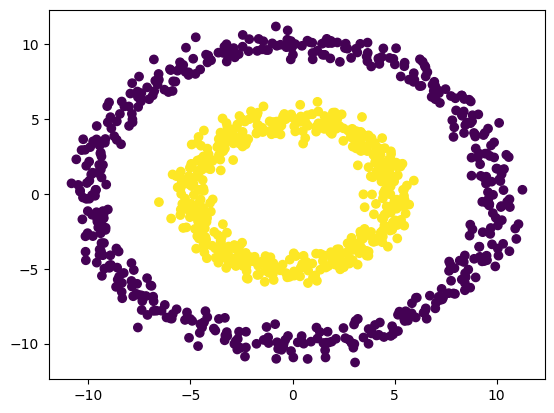
\includegraphics[width=\textwidth]{Spectral_Clustering_Images/concentric_circles_normalized.png}
         \end{minipage}
        \hfill
        \begin{minipage}[b]{0.4\textwidth}
            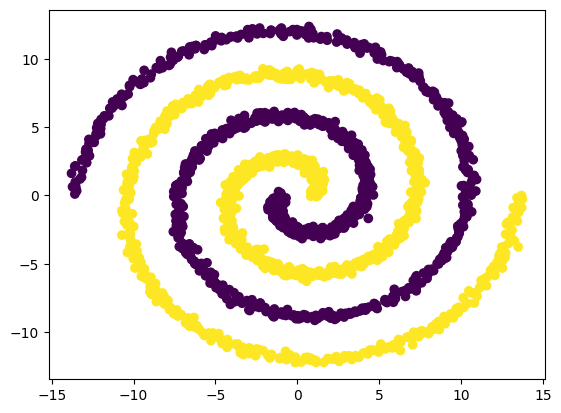
\includegraphics[width=\textwidth]{Spectral_Clustering_Images/interlacing_spirals_unnormalized.png}
        \end{minipage}
        \caption{Images were produced, from left to right, by normalized and unnormalized spectral clustering, respectively.}
    \end{figure}
\end{frame}


\begin{frame}{Disadvantages of Spectral Clustering}
    \begin{itemize}
        \item Sensitive to choice of similarity measure and its parameters, i.e. $\sigma$ in the Gaussian similarity measure
        \item The number of clusters $k$ must be pre-determined
    \end{itemize}
\end{frame}

\begin{frame}[fragile]{Implementation}
\begin{python}
def L_D_W_matrices(X, sigma = 1):
    #N = number of data points
    N = np.shape(X)[0]

    #Pairwise euclidean distances between all data points
    distances = euclidean_distances(X, X)

    #Compute the similarity matrix using the Gaussian similarity kernel
    gamma = 1.0 / (2 * sigma ** 2)
    W = np.exp(-gamma * distances ** 2)

    D = np.diag(np.sum(W, axis = 1))

    L = D - W

    return L, D, W
\end{python}

\end{frame}

\begin{frame}[fragile]{Implementation (Cont.)}
    \begin{python}
def normalized_spectral_clustering(X, k, sigma = 1):
    L, D, _ = L_D_W_matrices(X, sigma)
    N = np.shape(X)[0]

    #Solve generalized evec prob Lv = lambda Dv
    #These evecs are the evecs of I-D^{-1}W
    evals, evecs = eig(L, D)
    #Sort evals and evecs with evals increasing
    idx = np.argsort(evals.real)
    elvas = evals[idx]
    evecs = evecs[:,idx]

    #V houses the k evecs associated to smallest evals.
    V = evecs[:, :k]
    #Perform kmeans clustering on V
    kmeans = KMeans(n_clusters=k, random_state=0, n_init="auto").fit(V)

    return kmeans.labels_

    \end{python}
\end{frame}

\begin{frame}[fragile]{Implementation: Built-In Function}
\begin{python}
spectral_clustering = SpectralClustering(n_clusters=k, affinity='precomputed', random_state=0)
labels = spectral_clustering.fit_predict(W)
\end{python}
   \begin{figure}
        \begin{minipage}[b]{0.4\textwidth}
            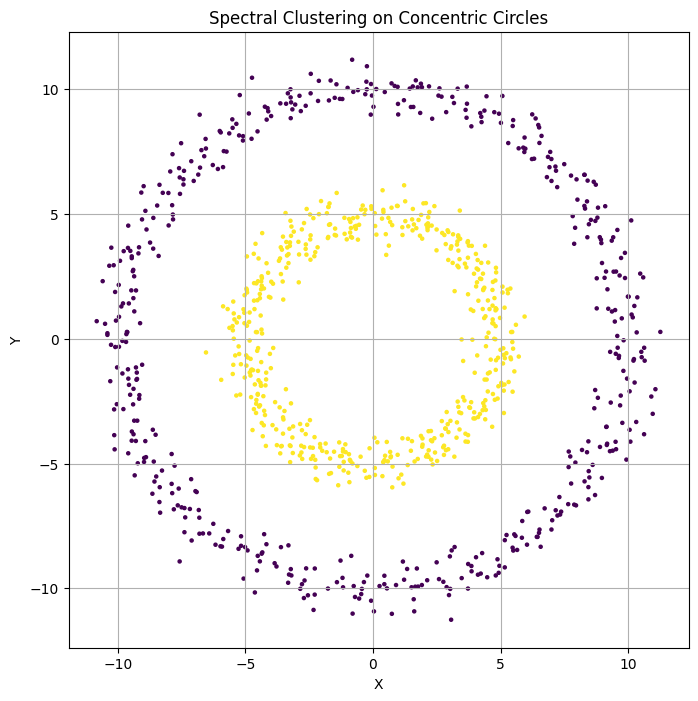
\includegraphics[width=\textwidth]{Spectral_Clustering_Images/concentric_circles_builtin.png}
         \end{minipage}
        \hfill
        \begin{minipage}[b]{0.4\textwidth}
            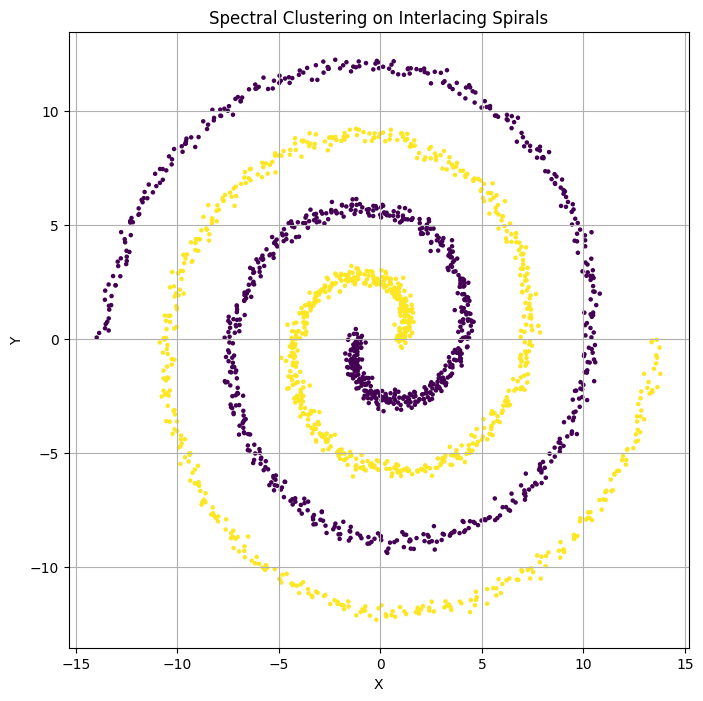
\includegraphics[width=\textwidth]{Spectral_Clustering_Images/interlacing_spirals_builtin.png}
        \end{minipage}
        \caption{Images were produced, from left to right, by normalized and unnormalized spectral clustering, respectively.}
    \end{figure}
\end{frame}
%%%%%%%%%%%%%%%%%%%%%%%%%%%%%%%%%%%%%%%%%%%%%%%%%%%%%%

\begin{frame}
    \begin{center}
      \textcolor{TennesseeOrange}{\huge Hierarchical Clustering}  
    \end{center}
\end{frame}
%%%%%%%%%%%%%%%%%%%%%%%%%%%%%%Roxana%%%%%%%%%%%%%%%%%%%%%%%%
\begin{frame}{Overview}
    \begin{outline} %Start with $N$ data points.
        \1 Agglomerative Hierarchical Clustering (AHC): Create a hierarchy by first considering each individual data point to be in its own cluster and at each step merging the clusters which are most similar. Eventually, all data points will be merged into one cluster. 
        \1 Divisive Hierarchical Clustering (DHC): Create a hierarchy by first considering all data points to be in the same cluster and at each step split the farthest point in the cluster. Eventually, all data points will be isolated in their own cluster. 
    \end{outline}
    The order of aggregating/dividing clusters is recorded in a dendrogram, which establishes a hierarchy in which data points are most similar.
\end{frame}

%\begin{frame}{Algorithm}
 %   \begin{enumerate}
  %      \item Compute the proximity matrix using a particular distance metric.
  %      \item Assign each data point to a cluster
  %      \item Merge (agglomerative) or divide (divisive) the clusters based on a chosen metric
  %      \item Update the proximity matrix
   %     \item Repeat Step 3 and Step 4 until only a single cluster remains (agglomerative) or until each data point is assigned to its own cluster (divisive)
  %  \end{enumerate}
%\end{frame}

%\begin{frame}{Proximity Matrix} 
 %   \begin{outline}
  %      \1 Given $N$ data points $x_1, \dots, x_N$, we define a $N \times N$ proximity matrix $P$ where $P_{i,j} = d(x_i, x_j)$.
  %      \2 The euclidean distance is a common distance metric used.
  %  \end{outline}
%\end{frame}

\begin{frame}{Dissimilarity Matrix}
A dissimilarity matrix $D$ is a matrix where $d_{i,i} = 0$ and $d_{i,j}\geq 0$ is a measure of ``distance'' between objects $i$ and $j$. 
\begin{itemize}
\item If we have a similarity matrix $S$, we
can convert it to a dissimilarity matrix by applying any monotonically decreasing function, e.g., $D=max(S)-S$.
%\item The euclidean distance is a common distance metric used.
\end{itemize}
\end{frame}





\begin{frame}{Algorithm}
\begin{figure}
        \centering
        \includegraphics[scale=0.6]{aglo_alg_diag.png}
        \label{fig:enter-label}
        \caption{Flow chart Agglomerative clustering}
\end{figure}
\end{frame}



%\begin{frame}{Aglomerative Clustering}
% \begin{figure}
 %       \centering
 %       \includegraphics[scale=0.5]{aglom_clust_alg.png}
 %       \label{fig:enter-label}
%\end{figure}
 %   The merging process can be represented as a binary tree called dendogram.
%\end{frame}

\begin{frame}{Types of Agglomerative Clustering}
 There are different variants of agglomerative clustering, depending on how we define
the dissimilarity between groups of objects. \\\vspace{0.5cm}
These can give quite different results. Three examples are:\\\vspace{0.5cm}
\begin{itemize}
    \item Single link
    \item Complete link
    \item Average link
\end{itemize}

\end{frame}

\begin{frame}{Agglomerative Clustering: Single Link}
 In single link clustering, also called nearest neighbor clustering, the distance between two groups $G$ and $H$ is defined as the distance between the two closest members of each group:
\[d_{SL}(G,H)=min_{i\in G, i'\in H} d_{i,i'}\]
 \begin{figure}
        \centering
        \includegraphics[scale=0.5]{aglo_clust_single_link.png}
        \label{fig:enter-label}
\end{figure}
\begin{itemize}
    \item Advantage: can accurately handle non-elliptical shapes
    \item Disadvantage: sensitive to noise and outliers
\end{itemize}
\end{frame}

\begin{frame}{Agglomerative Clustering: Complete Link}
In complete link clustering, also called furthest neighbor clustering, the distance between
two groups is defined as the distance between the two most distant pairs:
$$d_{CL}(G,H)=max_{i\in G, i'\in H} d_{i,i'}$$
 \begin{figure}
        \centering
        \includegraphics[scale=0.5]{aglo_clust_compl_link.png}
        \label{fig:enter-label}
\end{figure}
\begin{itemize}
    \item Advantage: less sensitive to noise than min link
    \item Disadvantage: can break large clusters and tends to be biased towards globular clusters
\end{itemize}
\end{frame}

\begin{frame}{Agglomerative Clustering: Average Link}
In practice, the preferred method is average link clustering, which measures the average
distance between all pairs:
$$d_{avg}(G,H)=\frac{1}{n_G n_H}\sum_{i\in G}\sum_{ i'\in H} d_{i,i'}$$
where $n_G$ and $n_H$ are the number of elements in groups $G$ and $H$.
 \begin{figure}
        \centering
        \includegraphics[scale=0.5]{aglo_clust_avr_link.png}
        \label{fig:enter-label}
\end{figure}
%\begin{itemize}
    %\item This method is less susceptible to noise and outliers than the other methods which seek to minimize the distance-based measurements
%\end{itemize}
\end{frame}

%\begin{frame}{Agglomerative Clustering: Ward Link}
%In this method the distance
%between two clusters is related to how much the sum of squares increases when the two clusters are combined:
%\begin{align*}
%    ESS(G) &= \sum_{i=1}^{N_G} \left|g_i - \frac{1}{N_G} \sum_{j=1}^{N_G}g_j \right|^2 \\
%    TD_{G \bigcup H} &= ESS(GH) - \left( ESS(G) + ESS(H) \right)
%\end{align*}
%$$TD_{G\cup H}=\sum_{i\in G\cup H} d_{i,\mu_{G\cup H}}$$
% \begin{figure}
%        \centering
%        \includegraphics[scale=0.3]{aglo_clust_ward_link.png}
%        \label{fig:enter-label}
%\end{figure}
%\begin{itemize}
%    \item This method is less susceptible to noise and outliers than the other methods which seek to minimize the distance-based measurements
%\end{itemize}
%\end{frame}
\begin{frame}{Divisive Clustering}
\begin{figure}
        \centering
        \includegraphics[scale=0.6]{div_alg_diag.png}
        \label{fig:enter-label}
        \caption{Flow chart Divisive clustering}
\end{figure}
%Starts with all the data in a single cluster, and then recursively divides each
%cluster into two daughter clusters, in a top-down fashion. \\
%Since there are $2^{N-1}-1$ ways to split
%a group of $N$ items into 2 groups, it is hard to compute the optimal split, so various heuristics
%are used. 
\end{frame}



%\begin{frame}{Divisive Clustering: Dissimilarity analysis approach}
%\begin{enumerate}
 %   \item Start with a single cluster containing all the data, $G = {1, . . . , N}$.
%    \item Measure the average dissimilarity of $i \in G$ to all the other $i' \in G$: 
%    $d_i^G=\frac{1}{n_G}\sum_{i'\in G} d_{i,i'}$
%    \item Remove the most dissimilar object and put it in its own cluster H: $i^{*}=arg\, max_{i\in G}d_i^{G}-d_i^{H}$, $G=G\backslash H$, $H=\{i^{*}\}$. 
 %   \begin{itemize}
 %       \item Specifically, we pick a point $i^*$ to move that maximizes the average dissimilarity to each $i' \in G$ but minimizes the average dissimilarity to each $i' \in H$: 
       %$$d_i^H=\frac{1}{n_H}\sum_{i'\in H} %d_{i,i'},\,i^{*}=arg\, max_{i\in G}d_i^{G}-%d_i^{H}$$, 
%    \end{itemize}
 %   \item Continue until $d_i^{G}-d_i^{H}$ is negative
%\end{enumerate} 
%\begin{itemize}
%\item The final result is that we have split G into
%two daughter clusters, G and H.
%\item Continue until the average dissimilarity within each cluster is below some threshold, and/or all clusters are singletons.
%\end{itemize}
%\end{frame}
%\begin{frame}{How it works?}
%\begin{itemize}
 %   \item In the first iteration, all points are assigned to a single cluster.
 %   \item In the second iteration, the single cluster is broken down into two smaller clusters.
 %   \item In the third iteration, it further breaks down into even smaller clusters.
 %   \item And so on it continues, until every point becomes a cluster itself.
%\end{itemize}
%\begin{figure}
 %       \centering
%        \includegraphics[scale=0.4]{divisive_hier.png}
%        \label{fig:enter-label}
%\end{figure}
%\end{frame}















%\begin{frame}{Step 3: Merge/Divide Clusters}
 %   \begin{outline}
  %      \1  To perform this step, you need to find a way to measure the distance between clusters. 
   %     \1 Can define cluster distance as:
    %        \2 the distance between the two closest members of each cluster (min or single link)
     %           \3 Advantage: can accurately handle non-elliptical shapes
      %          \3 Disadvantage: sensitive to noise and outliers
       %     \2 the distance between the two farthest members of each cluster (max or complete link)
        %        \3 Advantage: less sensitive to noise than min link
         %       \3 Disadvantage: can break large clusters and tends to be biased towards globular clusters
          %  \2 the average distance of all pairs in each cluster (average link)
           % \2 the distance between the centroids of the clusters (centroid link)
    %\end{outline}
%\end{frame}

%\begin{frame}{Step 3: Merge/Divide Clusters}
%    A different metric is the ward linkage, in which the distance between two clusters is related to how much the sum of squares increases when the two clusters are combined. \\ \vspace{0.25 cm}
 %   This method is less susceptible to noise and outliers than the other methods which seek to minimize the distance-based measurements.
%\end{frame}
%%%%%%%%%%%%%%%%%%%%%%%%%%%%%%%%%%%%%%%%%%%%%%%%%%%%%%%%%%%
%%%%%%%%%%%%%%%%%%%%%%%%%%%%%%%Charlotte%%%%%%%%%%%%%%%%%%
\begin{frame}{Dendrogram}
    Once the dendrogram is obtained, you select a threshold to determine the number of clusters and the membership in each cluster. \\
       \begin{figure}
            \begin{minipage}[b]{0.48\textwidth}
                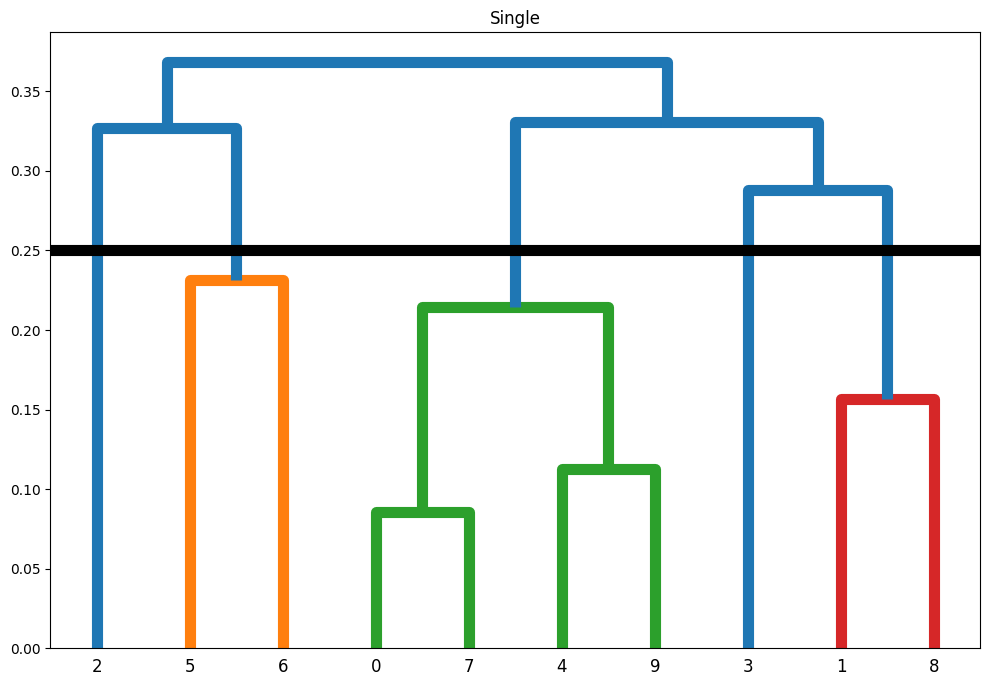
\includegraphics[width=\textwidth]{Dendrograms/single_linkage_dendrogram.png}
             \end{minipage}
            \hfill
            \begin{minipage}[b]{0.48\textwidth}
                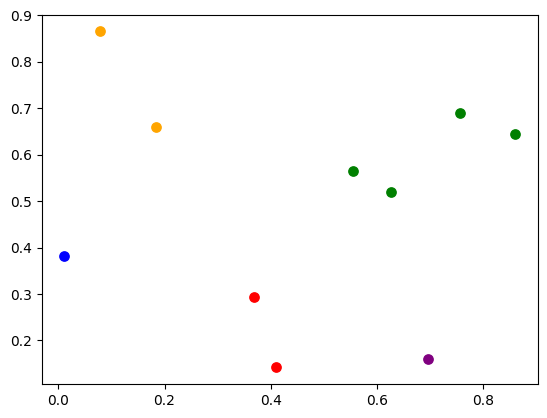
\includegraphics[width=\textwidth]{Dendrograms/single_linkage_clusters.png}
            \end{minipage}
        \end{figure}
    
     For example, in the provided image, for Single Linkage, a threshold of 0.25 produces five clusters because it intersects in five branches.
\end{frame}

\begin{frame}{Comparison of Different Linkages}
    \begin{figure}
        \centering
        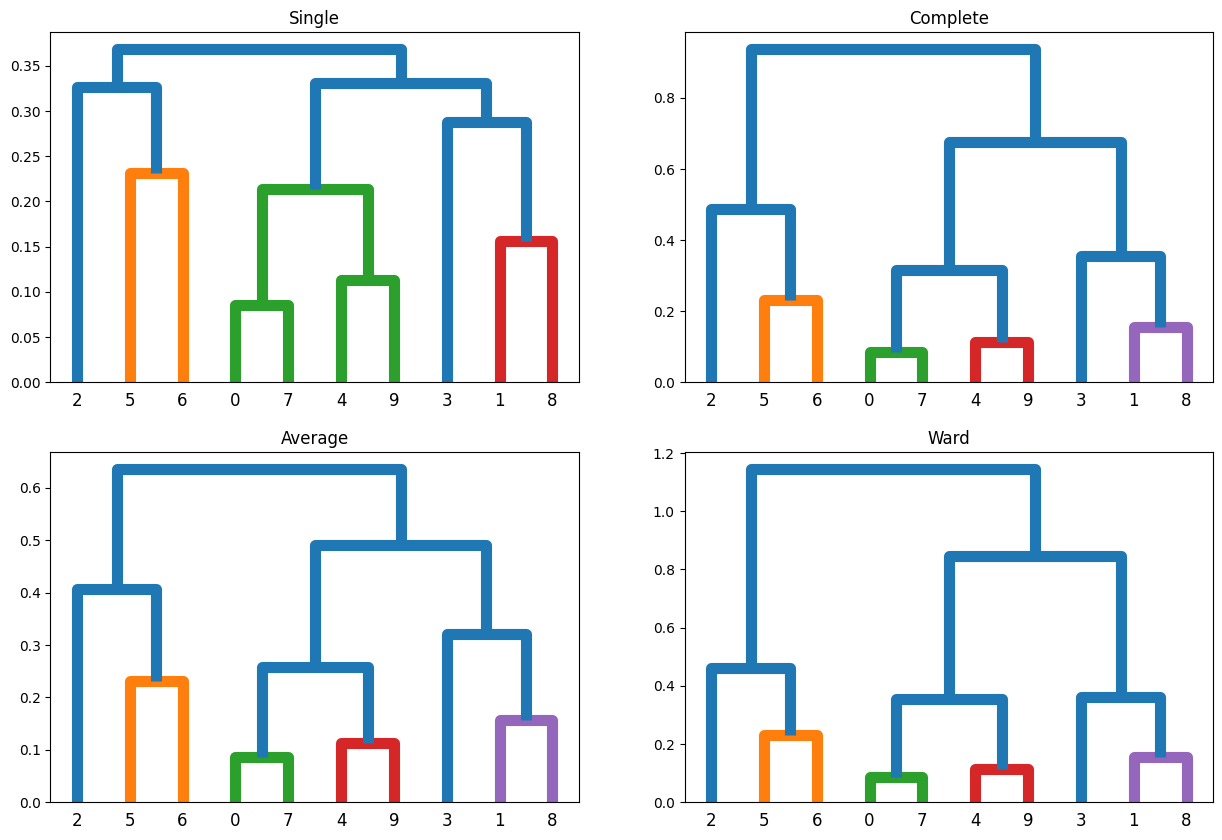
\includegraphics[scale=0.3]{Dendrograms/comparison_different_linkages.png}
        \caption{Different linkages can produce different clusters, even with the same threshold or with same $k$.}
        \label{fig:enter-label}
    \end{figure}
\end{frame}
%%%%%%%%%%%%%%%%%%%%%%%%%%%%%%%%%%%%%%%%%%%%%%%%%%%%%%%%%%%
%%%%%%%%%%%%%%%%%%%%%%%%%%%%%%%Sarah%%%%%%%%%%%%%%%%%%  
    


%\begin{frame}{Why this algorithm works}
    
%\end{frame}

\begin{frame}{Advantages of Hierarchical Clustering}
    \begin{outline}
        \1 Unlike in the $k$-means or spectral clustering algorithms, don't have to choose the number of clusters $k$ to partition into at the beginning. This is an advantage because when presented with data you may not know the true number of clusters which exist.
        \1 Provides a hierarchy of clusters.
    \end{outline}
\end{frame}

\begin{frame}{Disadvantages of Hierarchical Clustering}
    \begin{outline}
        \1 May have imbalanced clusters.
    \end{outline}
\end{frame}

\begin{frame}[fragile]{Implementation - Agglomerative Clustering}
    \begin{python}
   def hierarchical_clustering(X, n_clusters=2):
    # Initialize each sample as a cluster
    clstrs = [[i] for i in range(n_samples)]
    while len(clstrs) > n_clusters:
        min_dist = float('inf')
        merge_indices = None

        # Calc pairwise distances between clusters
        for i in range(len(clstrs)):
            for j in range(i+1, len(clstrs)):
                dist = complete_linkage_distance(X, clstrs[i], clstrs[j])
                if dist < min_dist:
                    min_dist = dist
                    merge_indices = (i, j)
    \end{python}
\end{frame}
\begin{frame}[fragile]
\begin{python}
    #When for loop is complete, know the two clusters
    #with min distance: merge them. 
    cluster1 = clstrs[merge_indices[0]],
    cluster2 = clstrs[merge_indices[1]]
    clstrs.pop(max(merge_indices))
    clstrs.pop(min(merge_indices))
    clstrs.append(cluster1 + cluster2)
    
    #Assign labels to each sample based on clustering
    for i, cluster in enumerate(clstrs):
        for sample_index in cluster:
            labels[sample_index] = i

    #Calculate cluster centers
    for i, clst in enumerate(clstrs):
        cluster_centers[i] = np.mean(X[clst], axis=0)

    return labels, cluster_centers
    \end{python}
\end{frame}






\begin{frame}[fragile]{Implementation - Divisive Clustering}
\begin{python}
def _divide_cluster(self, X):
    #Initialize all points in same cluster
    clusters = [X]
    while len(clusters) < self.n_clusters:
    max_dist_cluster_indx = self._find_max_dist_clustr
                            (clusters, X)
    max_dist_cluster = clusters[max_dist_cluster_indx]
    #Remove furthest point
    del clusters[max_dist_cluster_index]
    subclusters = self._bisect(max_dist_cluster) 
    clusters.extend(subclusters)
    self.labels = np.zeros(X.shape[0])
    self.centroids = []
    for i, cluster in enumerate(clusters):
      self.labels[np.isin(X, cluster).all(axis=1)] = i
      self.centers.append(np.mean(cluster, axis=0))
\end{python}
\end{frame}

\begin{frame}[fragile]{Implementation - Divisive Clustering}
    \begin{python}
def _find_max_dist_clustr(self, clusters, X):
    '''
    Function to find the cluster that contains the 
    data point that will be separated from the
    totality  
    '''
    max_distance = float('-inf')
    max_dist_cluster_index = 0
    for i, cluster in enumerate(clusters):
    dist = self._max_pairwise_distance(cluster, X)
    if dist > max_distance:
        max_distance = dist
        max_dist_cluster_index = i
        return max_dist_cluster_index
    \end{python}
\end{frame}
 

\begin{frame}{Implementation - Divisive Clustering}
    \begin{figure}
    \centering
    \begin{minipage}{.4\textwidth}
      \centering
      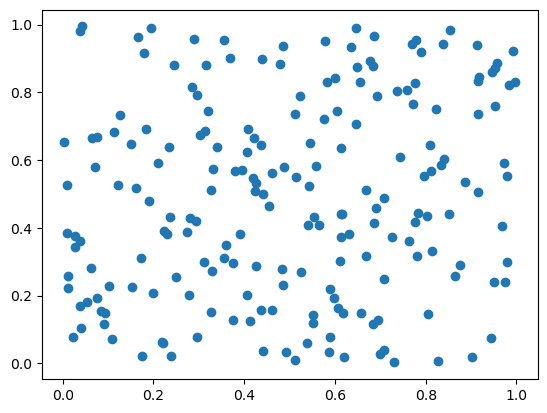
\includegraphics[width=\textwidth]{data_generation.png}
      \caption{Generated dataset}
      %\label{fig:test1}
    \end{minipage}
    \hfill
    \begin{minipage}{.4\textwidth}
      \centering
      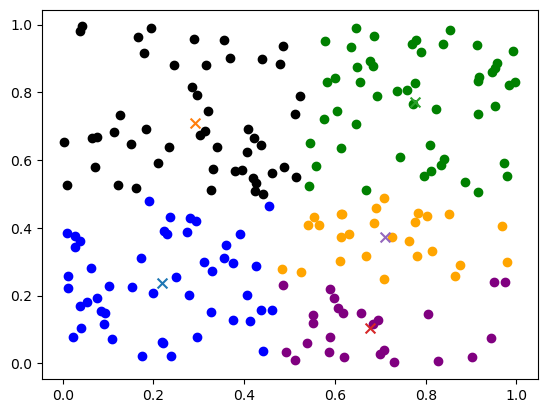
\includegraphics[width=\textwidth]{divisive_hierarchical_output.png}
      \caption{After divisive clustering}
      %\label{fig:test2}
    \end{minipage}
    \end{figure}
\end{frame}

\begin{frame}{Bayesian Approaches}
\begin{outline}
    \1 In 2023 Duan and Roy found that if a Bayesian spanning forest model is used as the distribution for the data points, the maximum likelihood estimate is almost the same as the point estimate from the normalized spectral clustering $(L_{\textrm{sym}})$. \vspace{0.5cm}
    \1 To learn about Bayesian hierarchical clustering, look at section 25.5.4 of Murphy's Machine Learning: A Probabilistic Perspective. 
    \2 Bayesian hierarchical clustering is similar to agglomerative clustering, but uses Bayesian hypothesis tests to decide which clusters to merge (if any).
\end{outline}
\end{frame}

\begin{frame}{Questions?}

    Code available on GitHub: https://github.com/sarahharkins7/Math526
\end{frame}

\begin{frame}
    \frametitle{References}
    \bibliographystyle{plain}
    {\footnotesize
    \bibliography{refs}}
    \nocite{*}
\end{frame}

%\begin{frame}{Spanning Forest Model}
%    \begin{outline}
%        \1 Suppose the data points $x_1, \dots x_N$ are clustered into $k$ groups $A_1, \dots, A_k$. \\
%        For each cluster, construct a component tree, $T_i$ (a connected subgraph without cycles). The set of nodes for each $T_i$ are the data points assigned to that cluster. Record the set of edges among those data points in the component tree.
%        \1 Let $\mathcal{A} = (T_1, \dots, T_k)$ be a forest graph.
%        \1 Using $\mathcal{F}_A$ and a set of root indices $\mathcal{R}_A = (1^*, \dots, K^*)$ with $k^* \in A_k$, they formed a graphical model with a conditional likelihood given the forest:
%        $$
%        \mathcal{L}(x; A, \mathcal{F}_A, \mathcal{R}_A, \theta) = \prod_{k=1}^K \left[r(x_{k^*}; \theta) \prod_{(i, j) \in T_k} f(x_i |x_j; \theta) \right]
%        $$
%        where $r(\cdot; \theta)$ is a ``root" distribution, $f(\cdot | y_j; \theta)$ is a ``leaf" distribution, $\theta$ denotes the other parameter, and $(i,j) \in T_k$ means that $(i, j)$ is an edge of the graph $T_k$.
%    \end{outline}
%\end{frame}

\end{document}
